\documentclass[twoside]{book}

% Packages required by doxygen
\usepackage{fixltx2e}
\usepackage{calc}
\usepackage{doxygen}
\usepackage[export]{adjustbox} % also loads graphicx
\usepackage{graphicx}
\usepackage[utf8]{inputenc}
\usepackage{makeidx}
\usepackage{multicol}
\usepackage{multirow}
\PassOptionsToPackage{warn}{textcomp}
\usepackage{textcomp}
\usepackage[nointegrals]{wasysym}
\usepackage[table]{xcolor}

% Font selection
\usepackage[T1]{fontenc}
\usepackage[scaled=.90]{helvet}
\usepackage{courier}
\usepackage{amssymb}
\usepackage{sectsty}
\renewcommand{\familydefault}{\sfdefault}
\allsectionsfont{%
  \fontseries{bc}\selectfont%
  \color{darkgray}%
}
\renewcommand{\DoxyLabelFont}{%
  \fontseries{bc}\selectfont%
  \color{darkgray}%
}
\newcommand{\+}{\discretionary{\mbox{\scriptsize$\hookleftarrow$}}{}{}}

% Page & text layout
\usepackage{geometry}
\geometry{%
  a4paper,%
  top=2.5cm,%
  bottom=2.5cm,%
  left=2.5cm,%
  right=2.5cm%
}
\tolerance=750
\hfuzz=15pt
\hbadness=750
\setlength{\emergencystretch}{15pt}
\setlength{\parindent}{0cm}
\setlength{\parskip}{3ex plus 2ex minus 2ex}
\makeatletter
\renewcommand{\paragraph}{%
  \@startsection{paragraph}{4}{0ex}{-1.0ex}{1.0ex}{%
    \normalfont\normalsize\bfseries\SS@parafont%
  }%
}
\renewcommand{\subparagraph}{%
  \@startsection{subparagraph}{5}{0ex}{-1.0ex}{1.0ex}{%
    \normalfont\normalsize\bfseries\SS@subparafont%
  }%
}
\makeatother

% Headers & footers
\usepackage{fancyhdr}
\pagestyle{fancyplain}
\fancyhead[LE]{\fancyplain{}{\bfseries\thepage}}
\fancyhead[CE]{\fancyplain{}{}}
\fancyhead[RE]{\fancyplain{}{\bfseries\leftmark}}
\fancyhead[LO]{\fancyplain{}{\bfseries\rightmark}}
\fancyhead[CO]{\fancyplain{}{}}
\fancyhead[RO]{\fancyplain{}{\bfseries\thepage}}
\fancyfoot[LE]{\fancyplain{}{}}
\fancyfoot[CE]{\fancyplain{}{}}
\fancyfoot[RE]{\fancyplain{}{\bfseries\scriptsize Generated by Doxygen }}
\fancyfoot[LO]{\fancyplain{}{\bfseries\scriptsize Generated by Doxygen }}
\fancyfoot[CO]{\fancyplain{}{}}
\fancyfoot[RO]{\fancyplain{}{}}
\renewcommand{\footrulewidth}{0.4pt}
\renewcommand{\chaptermark}[1]{%
  \markboth{#1}{}%
}
\renewcommand{\sectionmark}[1]{%
  \markright{\thesection\ #1}%
}

% Indices & bibliography
\usepackage{natbib}
\usepackage[titles]{tocloft}
\setcounter{tocdepth}{3}
\setcounter{secnumdepth}{5}
\makeindex

% Hyperlinks (required, but should be loaded last)
\usepackage{ifpdf}
\ifpdf
  \usepackage[pdftex,pagebackref=true]{hyperref}
\else
  \usepackage[ps2pdf,pagebackref=true]{hyperref}
\fi
\hypersetup{%
  colorlinks=true,%
  linkcolor=blue,%
  citecolor=blue,%
  unicode%
}

% Custom commands
\newcommand{\clearemptydoublepage}{%
  \newpage{\pagestyle{empty}\cleardoublepage}%
}

\usepackage{caption}
\captionsetup{labelsep=space,justification=centering,font={bf},singlelinecheck=off,skip=4pt,position=top}

%===== C O N T E N T S =====

\begin{document}

% Titlepage & ToC
\hypersetup{pageanchor=false,
             bookmarksnumbered=true,
             pdfencoding=unicode
            }
\pagenumbering{roman}
\begin{titlepage}
\vspace*{7cm}
\begin{center}%
{\Large Assignment 4 }\\
\vspace*{1cm}
{\large Generated by Doxygen 1.8.11}\\
\end{center}
\end{titlepage}
\clearemptydoublepage
\tableofcontents
\clearemptydoublepage
\pagenumbering{arabic}
\hypersetup{pageanchor=true}

%--- Begin generated contents ---
\chapter{Hierarchical Index}
\section{Class Hierarchy}
This inheritance list is sorted roughly, but not completely, alphabetically\+:\begin{DoxyCompactList}
\item \contentsline{section}{Card}{\pageref{class_card}}{}
\item exception\begin{DoxyCompactList}
\item \contentsline{section}{full}{\pageref{classfull}}{}
\item \contentsline{section}{invalid\+\_\+move}{\pageref{classinvalid__move}}{}
\item \contentsline{section}{not\+\_\+available}{\pageref{classnot__available}}{}
\end{DoxyCompactList}
\item \contentsline{section}{Foundation}{\pageref{class_foundation}}{}
\item \contentsline{section}{Free\+Cell}{\pageref{class_free_cell}}{}
\item \contentsline{section}{Setup}{\pageref{class_setup}}{}
\item \contentsline{section}{Tableau}{\pageref{class_tableau}}{}
\end{DoxyCompactList}

\chapter{Class Index}
\section{Class List}
Here are the classes, structs, unions and interfaces with brief descriptions\+:\begin{DoxyCompactList}
\item\contentsline{section}{\hyperlink{class_card}{Card} \\*Class representing a playing card }{\pageref{class_card}}{}
\item\contentsline{section}{\hyperlink{class_foundation}{Foundation} \\*Class representing a \hyperlink{class_foundation}{Foundation} pile in freecell }{\pageref{class_foundation}}{}
\item\contentsline{section}{\hyperlink{class_free_cell}{Free\+Cell} \\*Class representing the free cells in a \hyperlink{class_free_cell}{Free\+Cell} game }{\pageref{class_free_cell}}{}
\item\contentsline{section}{\hyperlink{classfull}{full} }{\pageref{classfull}}{}
\item\contentsline{section}{\hyperlink{classinvalid__move}{invalid\+\_\+move} }{\pageref{classinvalid__move}}{}
\item\contentsline{section}{\hyperlink{classnot__available}{not\+\_\+available} }{\pageref{classnot__available}}{}
\item\contentsline{section}{\hyperlink{class_setup}{Setup} }{\pageref{class_setup}}{}
\item\contentsline{section}{\hyperlink{class_tableau}{Tableau} \\*Class representing a \hyperlink{class_tableau}{Tableau} pile in freecell }{\pageref{class_tableau}}{}
\end{DoxyCompactList}

\chapter{File Index}
\section{File List}
Here is a list of all documented files with brief descriptions\+:\begin{DoxyCompactList}
\item\contentsline{section}{include/\hyperlink{_card_a_d_t_8h}{Card\+A\+D\+T.\+h} \\*Representing a playing card as an A\+DT }{\pageref{_card_a_d_t_8h}}{}
\item\contentsline{section}{include/\hyperlink{_exceptions_8h}{Exceptions.\+h} }{\pageref{_exceptions_8h}}{}
\item\contentsline{section}{include/\hyperlink{_foundation_8h}{Foundation.\+h} \\*Representing one of four foundation piles }{\pageref{_foundation_8h}}{}
\item\contentsline{section}{include/\hyperlink{_free_cell_8h}{Free\+Cell.\+h} \\*Representing one of four free cells }{\pageref{_free_cell_8h}}{}
\item\contentsline{section}{include/\hyperlink{_setup_8h}{Setup.\+h} \\*Representing the setup of the board and methods }{\pageref{_setup_8h}}{}
\item\contentsline{section}{include/\hyperlink{_tableau_8h}{Tableau.\+h} \\*Representing one of eight tableau piles }{\pageref{_tableau_8h}}{}
\end{DoxyCompactList}

\chapter{Class Documentation}
\hypertarget{class_card}{}\section{Card Class Reference}
\label{class_card}\index{Card@{Card}}


Class representing a playing card.  




{\ttfamily \#include $<$Card\+A\+D\+T.\+h$>$}

\subsection*{Public Member Functions}
\begin{DoxyCompactItemize}
\item 
\hyperlink{class_card_a1916ee0cda56d35edb572029ada2232c}{Card} (\hyperlink{_card_a_d_t_8h_adf74d53cd68bbef55ba510b266ecbbed}{Rank} rank, \hyperlink{_card_a_d_t_8h_af78e1c8ea5e6837b6ab9452a1e435e4e}{Suit} suit)
\begin{DoxyCompactList}\small\item\em Constructor for the \hyperlink{class_card}{Card} data type. \end{DoxyCompactList}\item 
\hyperlink{class_card_a783f5854cbe8c183ee3d4414c01472c0}{Card} ()\hypertarget{class_card_a783f5854cbe8c183ee3d4414c01472c0}{}\label{class_card_a783f5854cbe8c183ee3d4414c01472c0}

\begin{DoxyCompactList}\small\item\em creating constructor without parameter to dodge initialization \end{DoxyCompactList}\item 
\hyperlink{_card_a_d_t_8h_a7dae1270b9f323383fd77c3160a9927d}{Colour} \hyperlink{class_card_aaeb194c82f27e4256ae77deb5d89e335}{get\+Colour} ()
\begin{DoxyCompactList}\small\item\em returns the colour of the card \end{DoxyCompactList}\item 
\hyperlink{_card_a_d_t_8h_adf74d53cd68bbef55ba510b266ecbbed}{Rank} \hyperlink{class_card_aa517965f79ea53240c9208bbe4ec86be}{get\+Rank} ()
\begin{DoxyCompactList}\small\item\em returns rank of the card object \end{DoxyCompactList}\item 
\hyperlink{_card_a_d_t_8h_af78e1c8ea5e6837b6ab9452a1e435e4e}{Suit} \hyperlink{class_card_a3b1a0b15ea942b878d6344a1287c5351}{get\+Suit} ()
\begin{DoxyCompactList}\small\item\em returns suit of card \end{DoxyCompactList}\end{DoxyCompactItemize}


\subsection{Detailed Description}
Class representing a playing card. 

of a specific suit and rank. Colour is determined by suit 

\subsection{Constructor \& Destructor Documentation}
\index{Card@{Card}!Card@{Card}}
\index{Card@{Card}!Card@{Card}}
\subsubsection[{\texorpdfstring{Card(\+Rank rank, Suit suit)}{Card(Rank rank, Suit suit)}}]{\setlength{\rightskip}{0pt plus 5cm}Card\+::\+Card (
\begin{DoxyParamCaption}
\item[{{\bf Rank}}]{rank, }
\item[{{\bf Suit}}]{suit}
\end{DoxyParamCaption}
)}\hypertarget{class_card_a1916ee0cda56d35edb572029ada2232c}{}\label{class_card_a1916ee0cda56d35edb572029ada2232c}


Constructor for the \hyperlink{class_card}{Card} data type. 


\begin{DoxyParams}{Parameters}
{\em rank} & rank or value of card \\
\hline
{\em suit} & suit of card, one of the four suits \\
\hline
\end{DoxyParams}


\subsection{Member Function Documentation}
\index{Card@{Card}!get\+Colour@{get\+Colour}}
\index{get\+Colour@{get\+Colour}!Card@{Card}}
\subsubsection[{\texorpdfstring{get\+Colour()}{getColour()}}]{\setlength{\rightskip}{0pt plus 5cm}{\bf Colour} Card\+::get\+Colour (
\begin{DoxyParamCaption}
{}
\end{DoxyParamCaption}
)}\hypertarget{class_card_aaeb194c82f27e4256ae77deb5d89e335}{}\label{class_card_aaeb194c82f27e4256ae77deb5d89e335}


returns the colour of the card 

\begin{DoxyReturn}{Returns}
red or black depending on suit 
\end{DoxyReturn}
\index{Card@{Card}!get\+Rank@{get\+Rank}}
\index{get\+Rank@{get\+Rank}!Card@{Card}}
\subsubsection[{\texorpdfstring{get\+Rank()}{getRank()}}]{\setlength{\rightskip}{0pt plus 5cm}{\bf Rank} Card\+::get\+Rank (
\begin{DoxyParamCaption}
{}
\end{DoxyParamCaption}
)}\hypertarget{class_card_aa517965f79ea53240c9208bbe4ec86be}{}\label{class_card_aa517965f79ea53240c9208bbe4ec86be}


returns rank of the card object 

\begin{DoxyReturn}{Returns}
rank of card 
\end{DoxyReturn}
\index{Card@{Card}!get\+Suit@{get\+Suit}}
\index{get\+Suit@{get\+Suit}!Card@{Card}}
\subsubsection[{\texorpdfstring{get\+Suit()}{getSuit()}}]{\setlength{\rightskip}{0pt plus 5cm}{\bf Suit} Card\+::get\+Suit (
\begin{DoxyParamCaption}
{}
\end{DoxyParamCaption}
)}\hypertarget{class_card_a3b1a0b15ea942b878d6344a1287c5351}{}\label{class_card_a3b1a0b15ea942b878d6344a1287c5351}


returns suit of card 

\begin{DoxyReturn}{Returns}
suit of the card 
\end{DoxyReturn}


The documentation for this class was generated from the following file\+:\begin{DoxyCompactItemize}
\item 
include/\hyperlink{_card_a_d_t_8h}{Card\+A\+D\+T.\+h}\end{DoxyCompactItemize}

\hypertarget{class_foundation}{}\section{Foundation Class Reference}
\label{class_foundation}\index{Foundation@{Foundation}}


Class representing a \hyperlink{class_foundation}{Foundation} pile in freecell.  




{\ttfamily \#include $<$Foundation.\+h$>$}

\subsection*{Public Member Functions}
\begin{DoxyCompactItemize}
\item 
\hyperlink{class_foundation_a938dadcd731426c64fffc5798b7ca174}{Foundation} (\hyperlink{_card_a_d_t_8h_af78e1c8ea5e6837b6ab9452a1e435e4e}{Suit} suit)
\begin{DoxyCompactList}\small\item\em Constructor for a single foundation pile. \end{DoxyCompactList}\item 
void \hyperlink{class_foundation_ae1c591ca11d0a2841be8622323ed2b5f}{add\+Card} (\hyperlink{class_card}{Card} c)
\begin{DoxyCompactList}\small\item\em method for adding card onto foundation pile \end{DoxyCompactList}\item 
void \hyperlink{class_foundation_a7da4c5c94ab7d2d1f2fd2780c4d2172d}{remove\+Card} ()\hypertarget{class_foundation_a7da4c5c94ab7d2d1f2fd2780c4d2172d}{}\label{class_foundation_a7da4c5c94ab7d2d1f2fd2780c4d2172d}

\begin{DoxyCompactList}\small\item\em method for removing top card from foundation pile \end{DoxyCompactList}\item 
bool \hyperlink{class_foundation_a8d62650abd98bfbb229db88c2dc3381b}{is\+Full} ()
\begin{DoxyCompactList}\small\item\em checks if foundation pile is complete \end{DoxyCompactList}\item 
\hyperlink{_card_a_d_t_8h_af78e1c8ea5e6837b6ab9452a1e435e4e}{Suit} \hyperlink{class_foundation_a69fd10eded9c724eef919ea0efd5bb11}{get\+Suit} ()\hypertarget{class_foundation_a69fd10eded9c724eef919ea0efd5bb11}{}\label{class_foundation_a69fd10eded9c724eef919ea0efd5bb11}

\begin{DoxyCompactList}\small\item\em gets the suit of the foundation \end{DoxyCompactList}\item 
\hyperlink{class_card}{Card} \hyperlink{class_foundation_a22c3b4676d86b880e145731b2f0dc708}{top\+Card} ()\hypertarget{class_foundation_a22c3b4676d86b880e145731b2f0dc708}{}\label{class_foundation_a22c3b4676d86b880e145731b2f0dc708}

\begin{DoxyCompactList}\small\item\em gets the top card from the pile \end{DoxyCompactList}\end{DoxyCompactItemize}


\subsection{Detailed Description}
Class representing a \hyperlink{class_foundation}{Foundation} pile in freecell. 

that accepts a specific suit of cards 

\subsection{Constructor \& Destructor Documentation}
\index{Foundation@{Foundation}!Foundation@{Foundation}}
\index{Foundation@{Foundation}!Foundation@{Foundation}}
\subsubsection[{\texorpdfstring{Foundation(\+Suit suit)}{Foundation(Suit suit)}}]{\setlength{\rightskip}{0pt plus 5cm}Foundation\+::\+Foundation (
\begin{DoxyParamCaption}
\item[{{\bf Suit}}]{suit}
\end{DoxyParamCaption}
)}\hypertarget{class_foundation_a938dadcd731426c64fffc5798b7ca174}{}\label{class_foundation_a938dadcd731426c64fffc5798b7ca174}


Constructor for a single foundation pile. 


\begin{DoxyParams}{Parameters}
{\em suit} & suit of the cards belonging to the pile \\
\hline
\end{DoxyParams}


\subsection{Member Function Documentation}
\index{Foundation@{Foundation}!add\+Card@{add\+Card}}
\index{add\+Card@{add\+Card}!Foundation@{Foundation}}
\subsubsection[{\texorpdfstring{add\+Card(\+Card c)}{addCard(Card c)}}]{\setlength{\rightskip}{0pt plus 5cm}void Foundation\+::add\+Card (
\begin{DoxyParamCaption}
\item[{{\bf Card}}]{c}
\end{DoxyParamCaption}
)}\hypertarget{class_foundation_ae1c591ca11d0a2841be8622323ed2b5f}{}\label{class_foundation_ae1c591ca11d0a2841be8622323ed2b5f}


method for adding card onto foundation pile 


\begin{DoxyParams}{Parameters}
{\em c} & card being added to the pile \\
\hline
\end{DoxyParams}
\index{Foundation@{Foundation}!is\+Full@{is\+Full}}
\index{is\+Full@{is\+Full}!Foundation@{Foundation}}
\subsubsection[{\texorpdfstring{is\+Full()}{isFull()}}]{\setlength{\rightskip}{0pt plus 5cm}bool Foundation\+::is\+Full (
\begin{DoxyParamCaption}
{}
\end{DoxyParamCaption}
)}\hypertarget{class_foundation_a8d62650abd98bfbb229db88c2dc3381b}{}\label{class_foundation_a8d62650abd98bfbb229db88c2dc3381b}


checks if foundation pile is complete 

\begin{DoxyReturn}{Returns}
true if full, false otherwise 
\end{DoxyReturn}


The documentation for this class was generated from the following file\+:\begin{DoxyCompactItemize}
\item 
include/\hyperlink{_foundation_8h}{Foundation.\+h}\end{DoxyCompactItemize}

\hypertarget{class_free_cell}{}\section{Free\+Cell Class Reference}
\label{class_free_cell}\index{Free\+Cell@{Free\+Cell}}


Class representing the free cells in a \hyperlink{class_free_cell}{Free\+Cell} game.  




{\ttfamily \#include $<$Free\+Cell.\+h$>$}

\subsection*{Public Member Functions}
\begin{DoxyCompactItemize}
\item 
\hyperlink{class_free_cell_a4bba4f4932ee5ae1043aef8485116798}{Free\+Cell} ()\hypertarget{class_free_cell_a4bba4f4932ee5ae1043aef8485116798}{}\label{class_free_cell_a4bba4f4932ee5ae1043aef8485116798}

\begin{DoxyCompactList}\small\item\em constructor for \hyperlink{class_free_cell}{Free\+Cell} \end{DoxyCompactList}\item 
bool \hyperlink{class_free_cell_a96ff5f730b35c963e80a960352914147}{is\+Full} ()
\begin{DoxyCompactList}\small\item\em returns true if full, otehrwise false \end{DoxyCompactList}\item 
\hyperlink{class_card}{Card} \hyperlink{class_free_cell_af341fc1f3bdfc9edb7337879f12f45e6}{search\+Card} (\hyperlink{_card_a_d_t_8h_adf74d53cd68bbef55ba510b266ecbbed}{Rank} rank, \hyperlink{_card_a_d_t_8h_af78e1c8ea5e6837b6ab9452a1e435e4e}{Suit} suit)
\begin{DoxyCompactList}\small\item\em search for the card with the matching suit and rank \end{DoxyCompactList}\item 
void \hyperlink{class_free_cell_a31d2d73e75d6ca47531ab861e433ad03}{add\+Card} (\hyperlink{class_card}{Card} c)
\begin{DoxyCompactList}\small\item\em move card back to tableau or foundation \end{DoxyCompactList}\item 
void \hyperlink{class_free_cell_a8d41f669bf01f5c862121a4ff7d70ed8}{remove\+Card} (\hyperlink{_card_a_d_t_8h_adf74d53cd68bbef55ba510b266ecbbed}{Rank} rank, \hyperlink{_card_a_d_t_8h_af78e1c8ea5e6837b6ab9452a1e435e4e}{Suit} suit)
\begin{DoxyCompactList}\small\item\em remove card from free cells \end{DoxyCompactList}\end{DoxyCompactItemize}


\subsection{Detailed Description}
Class representing the free cells in a \hyperlink{class_free_cell}{Free\+Cell} game. 

\subsection{Member Function Documentation}
\index{Free\+Cell@{Free\+Cell}!add\+Card@{add\+Card}}
\index{add\+Card@{add\+Card}!Free\+Cell@{Free\+Cell}}
\subsubsection[{\texorpdfstring{add\+Card(\+Card c)}{addCard(Card c)}}]{\setlength{\rightskip}{0pt plus 5cm}void Free\+Cell\+::add\+Card (
\begin{DoxyParamCaption}
\item[{{\bf Card}}]{c}
\end{DoxyParamCaption}
)}\hypertarget{class_free_cell_a31d2d73e75d6ca47531ab861e433ad03}{}\label{class_free_cell_a31d2d73e75d6ca47531ab861e433ad03}


move card back to tableau or foundation 


\begin{DoxyParams}{Parameters}
{\em c} & card being added to free cells pile \\
\hline
\end{DoxyParams}
\index{Free\+Cell@{Free\+Cell}!is\+Full@{is\+Full}}
\index{is\+Full@{is\+Full}!Free\+Cell@{Free\+Cell}}
\subsubsection[{\texorpdfstring{is\+Full()}{isFull()}}]{\setlength{\rightskip}{0pt plus 5cm}bool Free\+Cell\+::is\+Full (
\begin{DoxyParamCaption}
{}
\end{DoxyParamCaption}
)}\hypertarget{class_free_cell_a96ff5f730b35c963e80a960352914147}{}\label{class_free_cell_a96ff5f730b35c963e80a960352914147}


returns true if full, otehrwise false 

\begin{DoxyReturn}{Returns}
true if all four cells are taken 
\end{DoxyReturn}
\index{Free\+Cell@{Free\+Cell}!remove\+Card@{remove\+Card}}
\index{remove\+Card@{remove\+Card}!Free\+Cell@{Free\+Cell}}
\subsubsection[{\texorpdfstring{remove\+Card(\+Rank rank, Suit suit)}{removeCard(Rank rank, Suit suit)}}]{\setlength{\rightskip}{0pt plus 5cm}void Free\+Cell\+::remove\+Card (
\begin{DoxyParamCaption}
\item[{{\bf Rank}}]{rank, }
\item[{{\bf Suit}}]{suit}
\end{DoxyParamCaption}
)}\hypertarget{class_free_cell_a8d41f669bf01f5c862121a4ff7d70ed8}{}\label{class_free_cell_a8d41f669bf01f5c862121a4ff7d70ed8}


remove card from free cells 


\begin{DoxyParams}{Parameters}
{\em rank} & rank of card being moved \\
\hline
{\em suit} & suit of card being moved \\
\hline
\end{DoxyParams}
\index{Free\+Cell@{Free\+Cell}!search\+Card@{search\+Card}}
\index{search\+Card@{search\+Card}!Free\+Cell@{Free\+Cell}}
\subsubsection[{\texorpdfstring{search\+Card(\+Rank rank, Suit suit)}{searchCard(Rank rank, Suit suit)}}]{\setlength{\rightskip}{0pt plus 5cm}{\bf Card} Free\+Cell\+::search\+Card (
\begin{DoxyParamCaption}
\item[{{\bf Rank}}]{rank, }
\item[{{\bf Suit}}]{suit}
\end{DoxyParamCaption}
)}\hypertarget{class_free_cell_af341fc1f3bdfc9edb7337879f12f45e6}{}\label{class_free_cell_af341fc1f3bdfc9edb7337879f12f45e6}


search for the card with the matching suit and rank 


\begin{DoxyParams}{Parameters}
{\em rank} & rank of card being moved \\
\hline
{\em suit} & suit of card being moved \\
\hline
\end{DoxyParams}


The documentation for this class was generated from the following file\+:\begin{DoxyCompactItemize}
\item 
include/\hyperlink{_free_cell_8h}{Free\+Cell.\+h}\end{DoxyCompactItemize}

\hypertarget{classfull}{}\section{full Class Reference}
\label{classfull}\index{full@{full}}
Inheritance diagram for full\+:\begin{figure}[H]
\begin{center}
\leavevmode
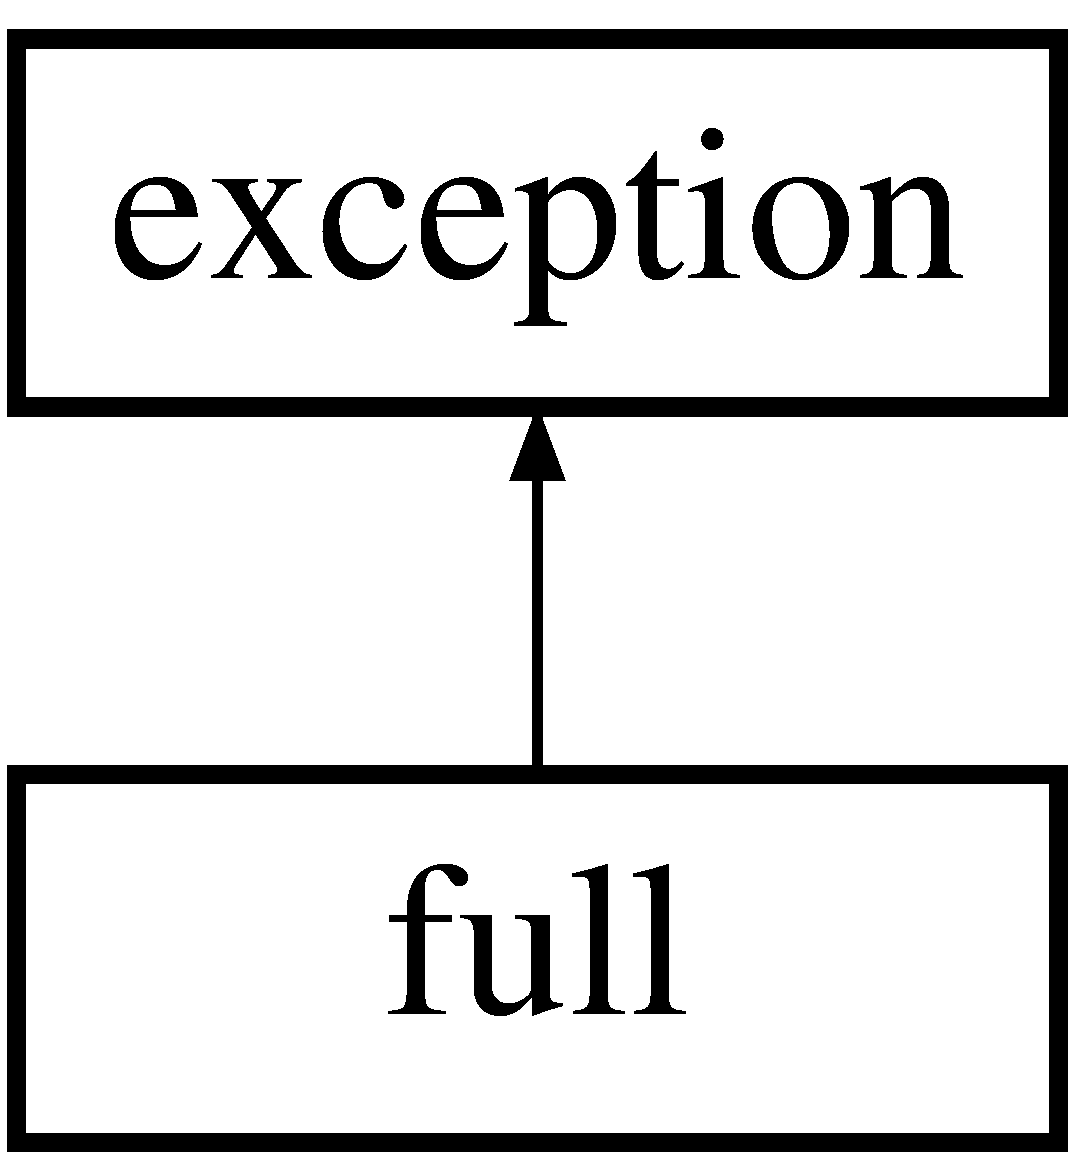
\includegraphics[height=2.000000cm]{classfull}
\end{center}
\end{figure}


The documentation for this class was generated from the following file\+:\begin{DoxyCompactItemize}
\item 
include/\hyperlink{_exceptions_8h}{Exceptions.\+h}\end{DoxyCompactItemize}

\hypertarget{classinvalid__move}{}\section{invalid\+\_\+move Class Reference}
\label{classinvalid__move}\index{invalid\+\_\+move@{invalid\+\_\+move}}
Inheritance diagram for invalid\+\_\+move\+:\begin{figure}[H]
\begin{center}
\leavevmode
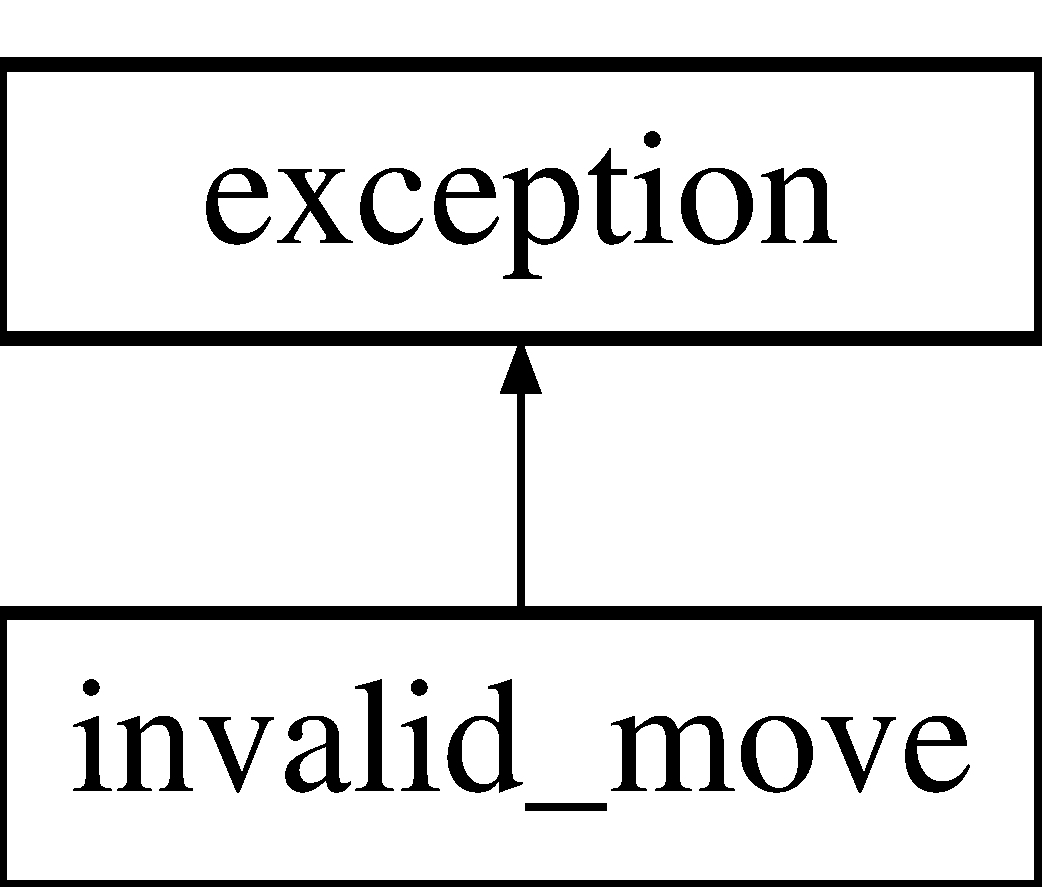
\includegraphics[height=2.000000cm]{classinvalid__move}
\end{center}
\end{figure}


The documentation for this class was generated from the following file\+:\begin{DoxyCompactItemize}
\item 
include/\hyperlink{_exceptions_8h}{Exceptions.\+h}\end{DoxyCompactItemize}

\hypertarget{classnot__available}{}\section{not\+\_\+available Class Reference}
\label{classnot__available}\index{not\+\_\+available@{not\+\_\+available}}
Inheritance diagram for not\+\_\+available\+:\begin{figure}[H]
\begin{center}
\leavevmode
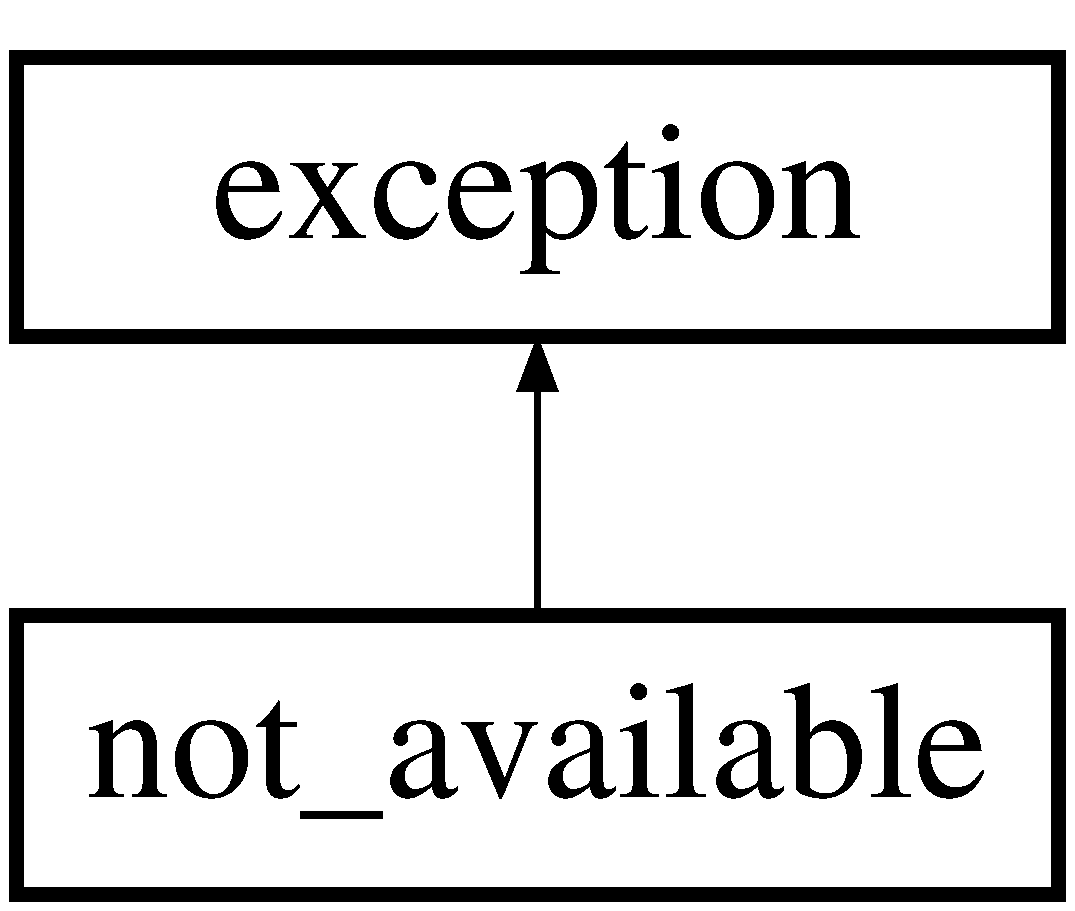
\includegraphics[height=2.000000cm]{classnot__available}
\end{center}
\end{figure}


The documentation for this class was generated from the following file\+:\begin{DoxyCompactItemize}
\item 
include/\hyperlink{_exceptions_8h}{Exceptions.\+h}\end{DoxyCompactItemize}

\hypertarget{class_setup}{}\section{Setup Class Reference}
\label{class_setup}\index{Setup@{Setup}}
\subsection*{Public Member Functions}
\begin{DoxyCompactItemize}
\item 
\hyperlink{class_setup_a0921e54e5a0200af117192e4c0c845b7}{Setup} ()
\item 
\hyperlink{class_setup_ae84ec0adca33996478fe9a226e6d2b2a}{Setup} (vector$<$ vector$<$ \hyperlink{class_card}{Card} $>$ $>$ s)
\item 
void \hyperlink{class_setup_a2b0bcfa40291817f662907720254d60b}{free\+To\+Tab} (\hyperlink{_card_a_d_t_8h_adf74d53cd68bbef55ba510b266ecbbed}{Rank} rank, \hyperlink{_card_a_d_t_8h_af78e1c8ea5e6837b6ab9452a1e435e4e}{Suit} suit, int to)
\begin{DoxyCompactList}\small\item\em moves card from the free cells to a teableau pile \end{DoxyCompactList}\item 
void \hyperlink{class_setup_ae424d4917db9cb013c904dbfcfa241e8}{tab\+To\+Tab} (int from, int to)
\begin{DoxyCompactList}\small\item\em moves card from the \hyperlink{class_tableau}{Tableau} \char`\"{}from\char`\"{} to the tableau \char`\"{}to\char`\"{} \end{DoxyCompactList}\item 
void \hyperlink{class_setup_a9356dbf0bccbfd14f5650297ef164479}{tab\+To\+Found} (int from)
\begin{DoxyCompactList}\small\item\em moves card from the \hyperlink{class_tableau}{Tableau} \char`\"{}from\char`\"{} to the foundation \end{DoxyCompactList}\item 
void \hyperlink{class_setup_a2d47948dfdaf388563bdcf090eb016e1}{tab\+To\+Free} (int from)
\begin{DoxyCompactList}\small\item\em moves card from the \hyperlink{class_tableau}{Tableau} \char`\"{}from\char`\"{} to a free cell \end{DoxyCompactList}\item 
void \hyperlink{class_setup_a109a5ee4d601011d72fe167c1acff07d}{free\+To\+Found} (\hyperlink{_card_a_d_t_8h_adf74d53cd68bbef55ba510b266ecbbed}{Rank} rank, \hyperlink{_card_a_d_t_8h_af78e1c8ea5e6837b6ab9452a1e435e4e}{Suit} suit)
\begin{DoxyCompactList}\small\item\em moves card from the free cells to foundation pile \end{DoxyCompactList}\item 
void \hyperlink{class_setup_a007aa7746a094ad3c435ded096dcfae5}{found\+To\+Tab} (\hyperlink{_card_a_d_t_8h_af78e1c8ea5e6837b6ab9452a1e435e4e}{Suit} suit, int to)
\begin{DoxyCompactList}\small\item\em moves top card from a foundation pile to tableau pile \end{DoxyCompactList}\item 
void \hyperlink{class_setup_a40e6d6ec8ee33bc01fef4a2a7367e218}{tab\+Top\+Cards} ()\hypertarget{class_setup_a40e6d6ec8ee33bc01fef4a2a7367e218}{}\label{class_setup_a40e6d6ec8ee33bc01fef4a2a7367e218}

\begin{DoxyCompactList}\small\item\em returns top cards on the tableau \end{DoxyCompactList}\item 
bool {\bfseries winning\+Game} ()\hypertarget{class_setup_a697c8770b52364a00510cd8fb8520ab5}{}\label{class_setup_a697c8770b52364a00510cd8fb8520ab5}

\end{DoxyCompactItemize}
\subsection*{Public Attributes}
\begin{DoxyCompactItemize}
\item 
\hyperlink{class_tableau}{Tableau} \hyperlink{class_setup_a4f1113264a61ae7746e07d4095cdac3f}{board} \mbox{[}8\mbox{]}\hypertarget{class_setup_a4f1113264a61ae7746e07d4095cdac3f}{}\label{class_setup_a4f1113264a61ae7746e07d4095cdac3f}

\begin{DoxyCompactList}\small\item\em 8 tableau piles \end{DoxyCompactList}\item 
\hyperlink{class_foundation}{Foundation} \hyperlink{class_setup_aaf0c941b751b10501560e6873db7636a}{founds} \mbox{[}4\mbox{]}\hypertarget{class_setup_aaf0c941b751b10501560e6873db7636a}{}\label{class_setup_aaf0c941b751b10501560e6873db7636a}

\begin{DoxyCompactList}\small\item\em 4 foundation piles \end{DoxyCompactList}\item 
\hyperlink{class_free_cell}{Free\+Cell} \hyperlink{class_setup_ade8fdfd786cd8782a0f2c5fb9519e9e3}{free}\hypertarget{class_setup_ade8fdfd786cd8782a0f2c5fb9519e9e3}{}\label{class_setup_ade8fdfd786cd8782a0f2c5fb9519e9e3}

\begin{DoxyCompactList}\small\item\em 4 free cells \end{DoxyCompactList}\end{DoxyCompactItemize}


\subsection{Constructor \& Destructor Documentation}
\index{Setup@{Setup}!Setup@{Setup}}
\index{Setup@{Setup}!Setup@{Setup}}
\subsubsection[{\texorpdfstring{Setup()}{Setup()}}]{\setlength{\rightskip}{0pt plus 5cm}Setup\+::\+Setup (
\begin{DoxyParamCaption}
{}
\end{DoxyParamCaption}
)}\hypertarget{class_setup_a0921e54e5a0200af117192e4c0c845b7}{}\label{class_setup_a0921e54e5a0200af117192e4c0c845b7}
Randomly constructs the initial state of the tableau piles and initializes freecells and foundation piles \index{Setup@{Setup}!Setup@{Setup}}
\index{Setup@{Setup}!Setup@{Setup}}
\subsubsection[{\texorpdfstring{Setup(vector$<$ vector$<$ Card $>$ $>$ s)}{Setup(vector< vector< Card > > s)}}]{\setlength{\rightskip}{0pt plus 5cm}Setup\+::\+Setup (
\begin{DoxyParamCaption}
\item[{vector$<$ vector$<$ {\bf Card} $>$ $>$}]{s}
\end{DoxyParamCaption}
)}\hypertarget{class_setup_ae84ec0adca33996478fe9a226e6d2b2a}{}\label{class_setup_ae84ec0adca33996478fe9a226e6d2b2a}
For manual set up of cards into tableaus 

\subsection{Member Function Documentation}
\index{Setup@{Setup}!found\+To\+Tab@{found\+To\+Tab}}
\index{found\+To\+Tab@{found\+To\+Tab}!Setup@{Setup}}
\subsubsection[{\texorpdfstring{found\+To\+Tab(\+Suit suit, int to)}{foundToTab(Suit suit, int to)}}]{\setlength{\rightskip}{0pt plus 5cm}void Setup\+::found\+To\+Tab (
\begin{DoxyParamCaption}
\item[{{\bf Suit}}]{suit, }
\item[{int}]{to}
\end{DoxyParamCaption}
)}\hypertarget{class_setup_a007aa7746a094ad3c435ded096dcfae5}{}\label{class_setup_a007aa7746a094ad3c435ded096dcfae5}


moves top card from a foundation pile to tableau pile 


\begin{DoxyParams}{Parameters}
{\em suit} & suit of card being moved \\
\hline
{\em to} & pile to which it is being moved \\
\hline
\end{DoxyParams}
\index{Setup@{Setup}!free\+To\+Found@{free\+To\+Found}}
\index{free\+To\+Found@{free\+To\+Found}!Setup@{Setup}}
\subsubsection[{\texorpdfstring{free\+To\+Found(\+Rank rank, Suit suit)}{freeToFound(Rank rank, Suit suit)}}]{\setlength{\rightskip}{0pt plus 5cm}void Setup\+::free\+To\+Found (
\begin{DoxyParamCaption}
\item[{{\bf Rank}}]{rank, }
\item[{{\bf Suit}}]{suit}
\end{DoxyParamCaption}
)}\hypertarget{class_setup_a109a5ee4d601011d72fe167c1acff07d}{}\label{class_setup_a109a5ee4d601011d72fe167c1acff07d}


moves card from the free cells to foundation pile 


\begin{DoxyParams}{Parameters}
{\em rank} & rank of card being moved \\
\hline
{\em suit} & suit of card being moved \\
\hline
\end{DoxyParams}
\index{Setup@{Setup}!free\+To\+Tab@{free\+To\+Tab}}
\index{free\+To\+Tab@{free\+To\+Tab}!Setup@{Setup}}
\subsubsection[{\texorpdfstring{free\+To\+Tab(\+Rank rank, Suit suit, int to)}{freeToTab(Rank rank, Suit suit, int to)}}]{\setlength{\rightskip}{0pt plus 5cm}void Setup\+::free\+To\+Tab (
\begin{DoxyParamCaption}
\item[{{\bf Rank}}]{rank, }
\item[{{\bf Suit}}]{suit, }
\item[{int}]{to}
\end{DoxyParamCaption}
)}\hypertarget{class_setup_a2b0bcfa40291817f662907720254d60b}{}\label{class_setup_a2b0bcfa40291817f662907720254d60b}


moves card from the free cells to a teableau pile 


\begin{DoxyParams}{Parameters}
{\em rank} & rank of card being moved \\
\hline
{\em suit} & suit of card being moved \\
\hline
{\em to} & index of tableau pile beng moved to \\
\hline
\end{DoxyParams}
\index{Setup@{Setup}!tab\+To\+Found@{tab\+To\+Found}}
\index{tab\+To\+Found@{tab\+To\+Found}!Setup@{Setup}}
\subsubsection[{\texorpdfstring{tab\+To\+Found(int from)}{tabToFound(int from)}}]{\setlength{\rightskip}{0pt plus 5cm}void Setup\+::tab\+To\+Found (
\begin{DoxyParamCaption}
\item[{int}]{from}
\end{DoxyParamCaption}
)}\hypertarget{class_setup_a9356dbf0bccbfd14f5650297ef164479}{}\label{class_setup_a9356dbf0bccbfd14f5650297ef164479}


moves card from the \hyperlink{class_tableau}{Tableau} \char`\"{}from\char`\"{} to the foundation 


\begin{DoxyParams}{Parameters}
{\em from} & pile from which a card is being moved to a free cell \\
\hline
\end{DoxyParams}
\index{Setup@{Setup}!tab\+To\+Free@{tab\+To\+Free}}
\index{tab\+To\+Free@{tab\+To\+Free}!Setup@{Setup}}
\subsubsection[{\texorpdfstring{tab\+To\+Free(int from)}{tabToFree(int from)}}]{\setlength{\rightskip}{0pt plus 5cm}void Setup\+::tab\+To\+Free (
\begin{DoxyParamCaption}
\item[{int}]{from}
\end{DoxyParamCaption}
)}\hypertarget{class_setup_a2d47948dfdaf388563bdcf090eb016e1}{}\label{class_setup_a2d47948dfdaf388563bdcf090eb016e1}


moves card from the \hyperlink{class_tableau}{Tableau} \char`\"{}from\char`\"{} to a free cell 


\begin{DoxyParams}{Parameters}
{\em from} & pile from which a card is being moved to foundation \\
\hline
\end{DoxyParams}
\index{Setup@{Setup}!tab\+To\+Tab@{tab\+To\+Tab}}
\index{tab\+To\+Tab@{tab\+To\+Tab}!Setup@{Setup}}
\subsubsection[{\texorpdfstring{tab\+To\+Tab(int from, int to)}{tabToTab(int from, int to)}}]{\setlength{\rightskip}{0pt plus 5cm}void Setup\+::tab\+To\+Tab (
\begin{DoxyParamCaption}
\item[{int}]{from, }
\item[{int}]{to}
\end{DoxyParamCaption}
)}\hypertarget{class_setup_ae424d4917db9cb013c904dbfcfa241e8}{}\label{class_setup_ae424d4917db9cb013c904dbfcfa241e8}


moves card from the \hyperlink{class_tableau}{Tableau} \char`\"{}from\char`\"{} to the tableau \char`\"{}to\char`\"{} 


\begin{DoxyParams}{Parameters}
{\em from} & pile from which a card is being moved \\
\hline
{\em to} & pile where card is dropped or appended \\
\hline
\end{DoxyParams}


The documentation for this class was generated from the following file\+:\begin{DoxyCompactItemize}
\item 
include/\hyperlink{_setup_8h}{Setup.\+h}\end{DoxyCompactItemize}

\hypertarget{class_tableau}{}\section{Tableau Class Reference}
\label{class_tableau}\index{Tableau@{Tableau}}


Class representing a \hyperlink{class_tableau}{Tableau} pile in freecell.  




{\ttfamily \#include $<$Tableau.\+h$>$}

\subsection*{Public Member Functions}
\begin{DoxyCompactItemize}
\item 
\hyperlink{class_tableau_a3cc548851797e21bea1bcaace6d0dc31}{Tableau} (vector$<$ \hyperlink{class_card}{Card} $>$ s)
\begin{DoxyCompactList}\small\item\em Constructor for \hyperlink{class_tableau}{Tableau}. \end{DoxyCompactList}\item 
void \hyperlink{class_tableau_a6d5eb19094e55901856cccb871066e52}{add\+Card} (\hyperlink{class_card}{Card} c)
\begin{DoxyCompactList}\small\item\em Adds card c to the tableau pile at hand. \end{DoxyCompactList}\item 
void \hyperlink{class_tableau_a6f27dda547e77b4a3ed7de954faf1d97}{remove\+Card} ()\hypertarget{class_tableau_a6f27dda547e77b4a3ed7de954faf1d97}{}\label{class_tableau_a6f27dda547e77b4a3ed7de954faf1d97}

\begin{DoxyCompactList}\small\item\em Removes top card from the current pile. \end{DoxyCompactList}\item 
\hyperlink{class_card}{Card} \hyperlink{class_tableau_a181138b61d0cadf5044f44712a45ccf9}{top\+Card} ()
\begin{DoxyCompactList}\small\item\em Extracts top card from pile. \end{DoxyCompactList}\end{DoxyCompactItemize}


\subsection{Detailed Description}
Class representing a \hyperlink{class_tableau}{Tableau} pile in freecell. 

where each card 

\subsection{Constructor \& Destructor Documentation}
\index{Tableau@{Tableau}!Tableau@{Tableau}}
\index{Tableau@{Tableau}!Tableau@{Tableau}}
\subsubsection[{\texorpdfstring{Tableau(vector$<$ Card $>$ s)}{Tableau(vector< Card > s)}}]{\setlength{\rightskip}{0pt plus 5cm}Tableau\+::\+Tableau (
\begin{DoxyParamCaption}
\item[{vector$<$ {\bf Card} $>$}]{s}
\end{DoxyParamCaption}
)}\hypertarget{class_tableau_a3cc548851797e21bea1bcaace6d0dc31}{}\label{class_tableau_a3cc548851797e21bea1bcaace6d0dc31}


Constructor for \hyperlink{class_tableau}{Tableau}. 

creates a tableau based on an input vector of cards 
\begin{DoxyParams}{Parameters}
{\em s} & a vector of 6 or 7 cards \\
\hline
\end{DoxyParams}


\subsection{Member Function Documentation}
\index{Tableau@{Tableau}!add\+Card@{add\+Card}}
\index{add\+Card@{add\+Card}!Tableau@{Tableau}}
\subsubsection[{\texorpdfstring{add\+Card(\+Card c)}{addCard(Card c)}}]{\setlength{\rightskip}{0pt plus 5cm}void Tableau\+::add\+Card (
\begin{DoxyParamCaption}
\item[{{\bf Card}}]{c}
\end{DoxyParamCaption}
)}\hypertarget{class_tableau_a6d5eb19094e55901856cccb871066e52}{}\label{class_tableau_a6d5eb19094e55901856cccb871066e52}


Adds card c to the tableau pile at hand. 


\begin{DoxyParams}{Parameters}
{\em c} & card being added to the pile \\
\hline
\end{DoxyParams}
\index{Tableau@{Tableau}!top\+Card@{top\+Card}}
\index{top\+Card@{top\+Card}!Tableau@{Tableau}}
\subsubsection[{\texorpdfstring{top\+Card()}{topCard()}}]{\setlength{\rightskip}{0pt plus 5cm}{\bf Card} Tableau\+::top\+Card (
\begin{DoxyParamCaption}
{}
\end{DoxyParamCaption}
)}\hypertarget{class_tableau_a181138b61d0cadf5044f44712a45ccf9}{}\label{class_tableau_a181138b61d0cadf5044f44712a45ccf9}


Extracts top card from pile. 

\begin{DoxyReturn}{Returns}
\hyperlink{class_card}{Card} object with the attributes of the card 
\end{DoxyReturn}


The documentation for this class was generated from the following file\+:\begin{DoxyCompactItemize}
\item 
include/\hyperlink{_tableau_8h}{Tableau.\+h}\end{DoxyCompactItemize}

\chapter{File Documentation}
\hypertarget{_card_a_d_t_8h}{}\section{include/\+Card\+A\+DT.h File Reference}
\label{_card_a_d_t_8h}\index{include/\+Card\+A\+D\+T.\+h@{include/\+Card\+A\+D\+T.\+h}}


Representing a playing card as an A\+DT.  


\subsection*{Classes}
\begin{DoxyCompactItemize}
\item 
class \hyperlink{class_card}{Card}
\begin{DoxyCompactList}\small\item\em Class representing a playing card. \end{DoxyCompactList}\end{DoxyCompactItemize}
\subsection*{Enumerations}
\begin{DoxyCompactItemize}
\item 
enum \hyperlink{_card_a_d_t_8h_af78e1c8ea5e6837b6ab9452a1e435e4e}{Suit} \{ {\bfseries C}, 
{\bfseries D}, 
{\bfseries S}, 
{\bfseries H}
 \}\hypertarget{_card_a_d_t_8h_af78e1c8ea5e6837b6ab9452a1e435e4e}{}\label{_card_a_d_t_8h_af78e1c8ea5e6837b6ab9452a1e435e4e}
\begin{DoxyCompactList}\small\item\em enum type for card suits in the order Clubs, Diamonds, spades and hearts respectively \end{DoxyCompactList}
\item 
enum \hyperlink{_card_a_d_t_8h_a7dae1270b9f323383fd77c3160a9927d}{Colour} \{ {\bfseries Red}, 
{\bfseries Black}
 \}\hypertarget{_card_a_d_t_8h_a7dae1270b9f323383fd77c3160a9927d}{}\label{_card_a_d_t_8h_a7dae1270b9f323383fd77c3160a9927d}
\begin{DoxyCompactList}\small\item\em enum type for card suit colour \end{DoxyCompactList}
\item 
enum \hyperlink{_card_a_d_t_8h_adf74d53cd68bbef55ba510b266ecbbed}{Rank} \{ \\*
{\bfseries Empty}, 
{\bfseries ace}, 
{\bfseries two}, 
{\bfseries three}, 
\\*
{\bfseries four}, 
{\bfseries five}, 
{\bfseries six}, 
{\bfseries seven}, 
\\*
{\bfseries eight}, 
{\bfseries nine}, 
{\bfseries ten}, 
{\bfseries jack}, 
\\*
{\bfseries queen}, 
{\bfseries king}
 \}\hypertarget{_card_a_d_t_8h_adf74d53cd68bbef55ba510b266ecbbed}{}\label{_card_a_d_t_8h_adf74d53cd68bbef55ba510b266ecbbed}
\begin{DoxyCompactList}\small\item\em enum type for card rank or value \end{DoxyCompactList}
\end{DoxyCompactItemize}


\subsection{Detailed Description}
Representing a playing card as an A\+DT. 

\begin{DoxyAuthor}{Author}
Andy Hameed $\vert$ 400073469
\end{DoxyAuthor}
along with enume types for card attributes 
\hypertarget{_exceptions_8h}{}\section{include/\+Exceptions.h File Reference}
\label{_exceptions_8h}\index{include/\+Exceptions.\+h@{include/\+Exceptions.\+h}}
{\ttfamily \#include $<$exception$>$}\\*
\subsection*{Classes}
\begin{DoxyCompactItemize}
\item 
class \hyperlink{classinvalid__move}{invalid\+\_\+move}
\item 
class \hyperlink{classfull}{full}
\item 
class \hyperlink{classnot__available}{not\+\_\+available}
\end{DoxyCompactItemize}


\subsection{Detailed Description}
\begin{DoxyAuthor}{Author}
Andy Hameed $\vert$ 400073469 
\end{DoxyAuthor}

\hypertarget{_foundation_8h}{}\section{include/\+Foundation.h File Reference}
\label{_foundation_8h}\index{include/\+Foundation.\+h@{include/\+Foundation.\+h}}


Representing one of four foundation piles.  


{\ttfamily \#include $<$vector$>$}\\*
\subsection*{Classes}
\begin{DoxyCompactItemize}
\item 
class \hyperlink{class_foundation}{Foundation}
\begin{DoxyCompactList}\small\item\em Class representing a \hyperlink{class_foundation}{Foundation} pile in freecell. \end{DoxyCompactList}\end{DoxyCompactItemize}


\subsection{Detailed Description}
Representing one of four foundation piles. 

\begin{DoxyAuthor}{Author}
Andy Hameed $\vert$ 400073469
\end{DoxyAuthor}
one for each suit 
\hypertarget{_free_cell_8h}{}\section{include/\+Free\+Cell.h File Reference}
\label{_free_cell_8h}\index{include/\+Free\+Cell.\+h@{include/\+Free\+Cell.\+h}}


Representing one of four free cells.  


{\ttfamily \#include $<$vector$>$}\\*
\subsection*{Classes}
\begin{DoxyCompactItemize}
\item 
class \hyperlink{class_free_cell}{Free\+Cell}
\begin{DoxyCompactList}\small\item\em Class representing the free cells in a \hyperlink{class_free_cell}{Free\+Cell} game. \end{DoxyCompactList}\end{DoxyCompactItemize}


\subsection{Detailed Description}
Representing one of four free cells. 

\begin{DoxyAuthor}{Author}
Andy Hameed $\vert$ 400073469 
\end{DoxyAuthor}

\hypertarget{_setup_8h}{}\section{include/\+Setup.h File Reference}
\label{_setup_8h}\index{include/\+Setup.\+h@{include/\+Setup.\+h}}


Representing the setup of the board and methods.  


{\ttfamily \#include $<$vector$>$}\\*
\subsection*{Classes}
\begin{DoxyCompactItemize}
\item 
class \hyperlink{class_setup}{Setup}
\end{DoxyCompactItemize}


\subsection{Detailed Description}
Representing the setup of the board and methods. 

\begin{DoxyAuthor}{Author}
Andy Hameed $\vert$ 400073469
\end{DoxyAuthor}
for changing the game state 
\hypertarget{_tableau_8h}{}\section{include/\+Tableau.h File Reference}
\label{_tableau_8h}\index{include/\+Tableau.\+h@{include/\+Tableau.\+h}}


Representing one of eight tableau piles.  


{\ttfamily \#include $<$vector$>$}\\*
\subsection*{Classes}
\begin{DoxyCompactItemize}
\item 
class \hyperlink{class_tableau}{Tableau}
\begin{DoxyCompactList}\small\item\em Class representing a \hyperlink{class_tableau}{Tableau} pile in freecell. \end{DoxyCompactList}\end{DoxyCompactItemize}


\subsection{Detailed Description}
Representing one of eight tableau piles. 

\begin{DoxyAuthor}{Author}
Andy Hameed $\vert$ 400073469 
\end{DoxyAuthor}

%--- End generated contents ---

% Index
\backmatter
\newpage
\phantomsection
\clearemptydoublepage
\addcontentsline{toc}{chapter}{Index}
\printindex

\end{document}
